\chapter{PPO Hyperparameters}
In this section are shown all the hyperparameters used for PPO algorithm depending on the different environment. All these were found by a manual tuning, so they aren't the optimal ones, but work well for the purpose of this thesis.\\Looking at the Tables below, the parameters stands for:
\begin{itemize}
    \item \textit{Max episode length}, is the maximum duration for an episode measured in timesteps
    \item \textit{Max training timesteps}, is the maximum duration of the total optimization process, after which the DT is returned to the main algorithm
    \item \textit{Update timestamp}, measures how often the optimization takes place (remember that PPO first takes data in order to evaluate in a second moment the actions and after that it applies the loss function for \textit{epochs} times)
    \item \textit{Epochs}, is the number of times that the backpropagation is done
    \item \textit{Epsilon clip parameter}, is a parameter for the surrogate clipped function in the loss function
    \item \textit{Gamma}, is the discount factor
    \item \textit{Learning rate actor/critic}, are the learning rates assigned to the actor/critic in the Actor-Critic model.
\end{itemize}

\begin{table}[h!]
\begin{center}
\begin{tabular}{ |c|c| } 
\hline
\textbf{Parameter} & \textbf{Value} \\
\hline
Max episode length & 500\\
Max training timesteps & $10^5$\\
Update timestamp & 3000\\
Epochs & 60\\
Epsilon clip parameter & 0.2\\
Gamma & 0.95\\
Learning rate actor & 0.001\\
Learning rate critic & 0.001\\
\hline
\end{tabular}
\caption{Parameters used for PPO in the CartPole-v1 environment}
\label{table:100}
\end{center}
\end{table}


\begin{table}[h!]
\begin{center}
\begin{tabular}{ |c|c| } 
\hline
\textbf{Parameter} & \textbf{Value} \\
\hline
Max episode length & 500\\
Max training timesteps & $10^5*1.5$\\
Update timestamp & 10000\\
Epochs & 15\\
Epsilon clip parameter & 0.2\\
Gamma & 0.95\\
Learning rate actor & 0.001\\
Learning rate critic & 0.001\\
\hline
\end{tabular}
\caption{Parameters used for PPO in the Acrobot-v0 environment}
\label{table:102}
\end{center}
\end{table}


\begin{table}[h!]
\begin{center}
\begin{tabular}{ |c|c| } 
\hline
\textbf{Parameter} & \textbf{Value} \\
\hline
Max episode length & 200\\
Max training timesteps & $10^5$\\
Update timestamp & 6000\\
Epochs & 20\\
Epsilon clip parameter & 0.2\\
Gamma & 0.95\\
Learning rate actor & 0.001\\
Learning rate critic & 0.001\\
\hline
\end{tabular}
\caption{Parameters used for PPO in the MountainCar-v1 environment}
\label{table:101}
\end{center}
\end{table}



\chapter{Complete Decision Trees and pruning method}
In this section are shown the complete version of the best trees before pruning them and it is also explained the pruning process.

\section{Full DTs}
\begin{figure}[h!]
    \centering
    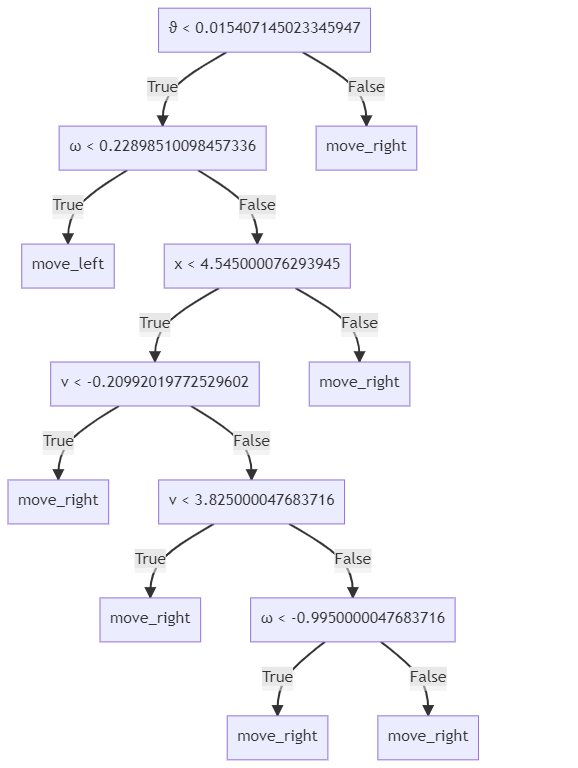
\includegraphics[width=0.7\linewidth]{images/CartPole/bestPPOcompleteCP.png}
    \caption{Full DT evolved by PPO for the CartPole-v1 environment}
    \label{fig:TreeFullCP}
\end{figure}

\begin{figure}[h!]
    \centering
    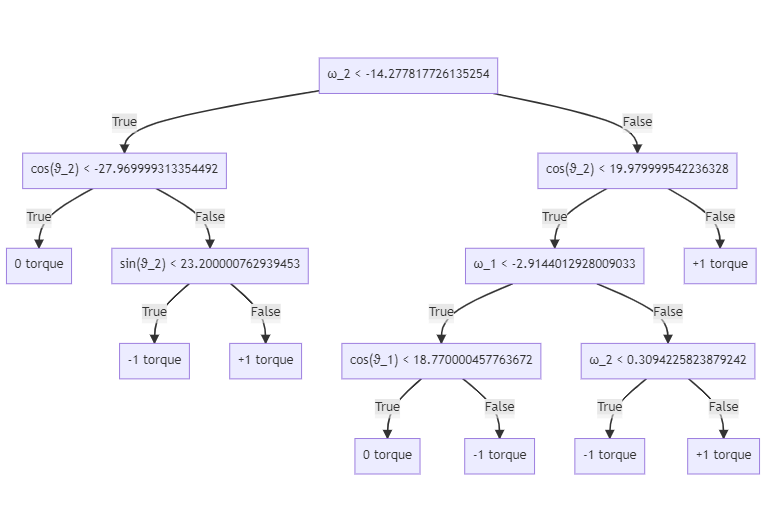
\includegraphics[width=0.7\linewidth]{images/Acrobot/bestPPOcompleteAB.png}
    \caption{Full DT evolved by PPO for the Acrobot-v1 environment}
    \label{fig:TreeFullAB}
\end{figure}

\begin{figure}[h!]
    \centering
    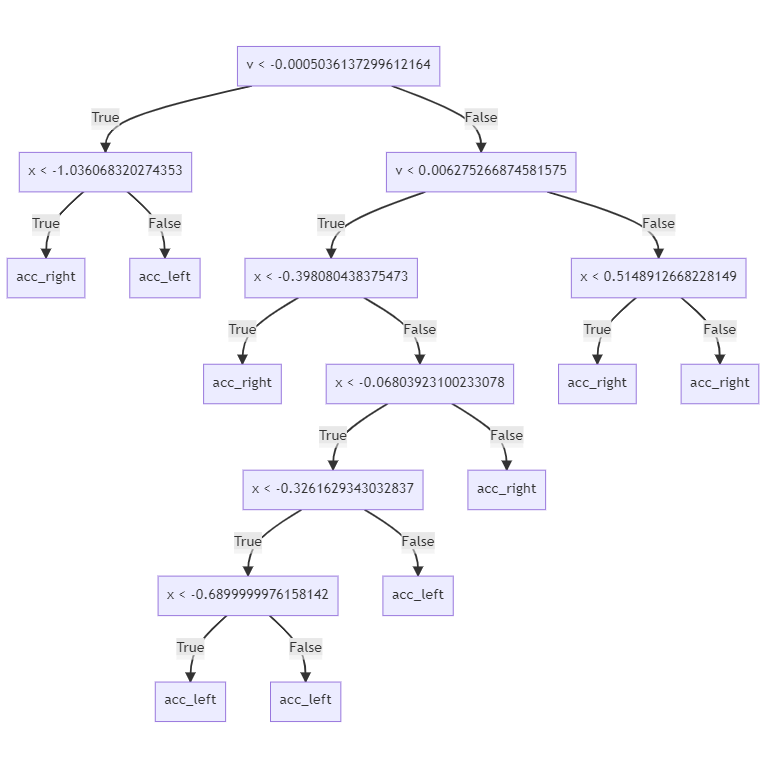
\includegraphics[width=0.7\linewidth]{images/MountainCar/bestPPOcompleteMC.png}
    \caption{Full DT evolved by PPO for the MountainCar-v0 environment}
    \label{fig:TreeFullMC}
\end{figure}

\newpage

\section{Pruning method}
\label{sec:prune}
To obtain the pruned DTs, I used a python code that tries the model in the environment for several times and marks every node that was visited. After this process, all the nodes that were not marked are eliminated and the tree is rearranged accordingly. To accentuate even more the fact that the models are highly interpretable and it's really easy and fast to prune them also by hand, I made a manual pruning of the DTs obtained in the followings subsections.

\subsection{CartPole-v1}
Considering the Figure \ref{fig:TreeFullCP} and the Subsection \ref{subsec:411} containing the constraints for the environment, starting from the root is possible to make the following considerations: the condition in the root is a valid one, so it's left untouched with its right child (a leaf). Proceeding with its left child, also this is a valid condition, so we can leave it with its left leaf. Moving now on its right child, here its possible to make a consideration to speed up the simplification process: every leaf in this subtree contains the same action, so it's possible to replace the whole subtree with a leaf containing the action in common to all the leaves (move\_right), finishing the process.

The final result is the DT shown in the Figure \ref{fig:BestTreeCP} which is quite easier to understand compared to the complete version (the split values were also rounded for a better visualization).



\subsection{Acrobot-v1}
Considering the Figure \ref{fig:TreeFullCP} and the Subsection \ref{subsec:421} containing the constraints for the environment, starting from the root is possible to make the following considerations: the root is a valid condition, so we can left it untouched.

Moving first on its left subtree, there's an invalid Boolean condition (a cosine always stands in the interval [-1,1]) and is always false: so we can connect its right subtree directly to the root; continuing on this condition, also this was pass the trigonometric boundaries and is evaluated every time as true: so we can link its left leaf to the root, removing all the conditions between, finishing the left subtree.

Proceeding on the right subtree of the root, there is a condition that is always true (passes the higher bound for cosine function): so we remove it with its right child, continuing with its left child, which is a valid condition. Despite this, its left child is an invalid condition (always true), so we can link to it the left leaf removing the condition in between. Finally, moving on its right subtree, there a valid Boolean condition.

Lastly, also the left subtree of the root is substituted with a leaf, because it's composed by a condition that lead to the same action, independently from the decision taken.

The final result is the DT shown in the Figure \ref{fig:BestTreeAB} (the split values were also rounded for a better visualization).


\subsection{MountainCar-v1}
Considering the Figure \ref{fig:TreeFullCP} and the Subsection \ref{subsec:421} containing the constraints for the environment, starting from the root is possible to make the following considerations: starting from the root, there's a valid condition, so we can leave it untouched.

Its left subtree is composed by a valid condition and 2 distinct leaves, so we can leave it untouched too.

Moving on the right subtree, we find another valid condition and also its right child is a valid condition, so there's nothing to prune here. Proceeding on the left, there's a valid condition, so it's left untouched with its left leaf. Passing on its right child, we can found a valid condition, but during the testing phases (tested on 100 unseen episode), it was found heuristically that this condition could not be false: for this reason, we can cut off it right child and connect its left subtree to its parent. Moving on the next condition, it's a valid one, so we can proceed with it's left child (the last condition); this condition is always evaluated as false due to the previous conditions: so we can remove it with its left child and connect its right leaf to its parent, finishing this process.

Lastly, we pass the tree removing all the double leaves, replacing them with its parent with a leaf containing the same action that was present in the previous leaves, concluding the pruning process.

The final result is the DT shown in the Figure \ref{fig:BestTreeMC} (the split values were also rounded for a better visualization).